\documentclass[a4paper]{article}

\usepackage[latin1]{inputenc}
\usepackage{amssymb}
\usepackage{framed}
\usepackage{graphicx}
\usepackage{subcaption}



\setlength{\parindent}{0pt}
\setlength{\parskip}{3ex}

\begin{document}

\begin{center}
  {\large Artificial Neural Networks and Deep Architectures, DD2437}\\
  \vspace{7mm}
  {\huge Short report on lab assignment 1\\[1ex]}
  {\Large Classification with a single-layer perceptron}\\
  \vspace{8mm}  
  {\Large Hasan Alzubeidi, Rakin Ali and Steinar Logi \\}
  \vspace{4mm}
  {\large January 22, 2024 \\}
\end{center}

\section{Main objectives and scope of the assignment \normalsize}
The main objective with this assignment is to familiarize ourselves with the perceptron learning rule and the delta learning rule along with batch versus sequential learning method. 
Our major goals in the assignment were  
\begin{itemize}
\item Implement and explore the perceptron learning rule for simple classification tasks
\item Implement and explore the delta learning rule for simple classification tasks 
\item Explore how the perceptron and delta learning rule performs on linearly separable data compare to a dataset that is not linearly separable
\item Explore how the bias affects the convergence of the delta learning algorithm
\end{itemize}

This assignment was scoped on the delta and perceptron learning rule. For the delta rule we used batch learning and sequential learning; for perceptron learning rule, we only used sequential learning. The limitations were the different learning rate

\section{Methods} This lab was conducted three separate times as we did not collaborate when writing the code. We all did the code separately then compared our results. The code was written in Jupyter notebook and regular python v3.9 file. We all drew more or less the same conclusions based on our results however got different graphs. Numpy function and matplot were the only libraries used.  \\

\section{Results and discussion}
\subsection{Classification with a single-layer perceptron}
\textbf{Perceptron versus Delta Rule Learning: }In this Section we compared two learning algorithms with a single perception. The algorithms compared were delta rule and perception learning. From the lectures we learned that perceptron learning converges to the "first best solution" it finds however that result does not generalize well compared to delta rule. This is evident in figure \ref{fig:Decision Boundary} as the boundary line generalizes better. Regarding convergence, delta rule converges faster as a lot less iterations were needed. 
\begin{figure}[htb]
    \centering
    \begin{subfigure}{0.4\textwidth}
        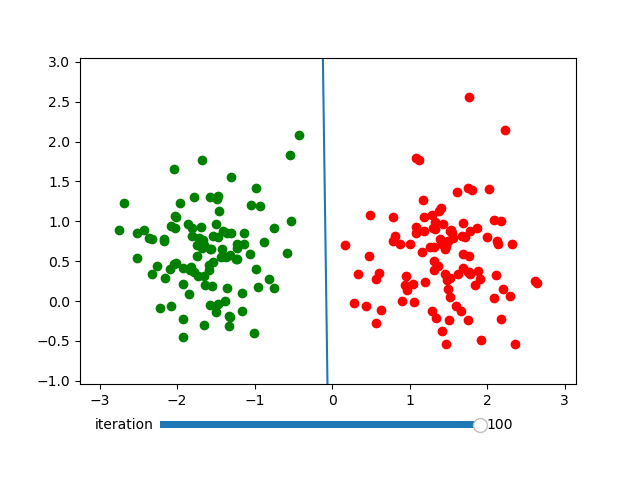
\includegraphics[width=\textwidth]{Labs/Lab 1/Lab 1a/Results/Delta-linear-seperable.png}
        \caption{Delta rule}
        \label{fig:Delta Rule}
    \end{subfigure}
    \hfill
    \begin{subfigure}{0.4\textwidth}
        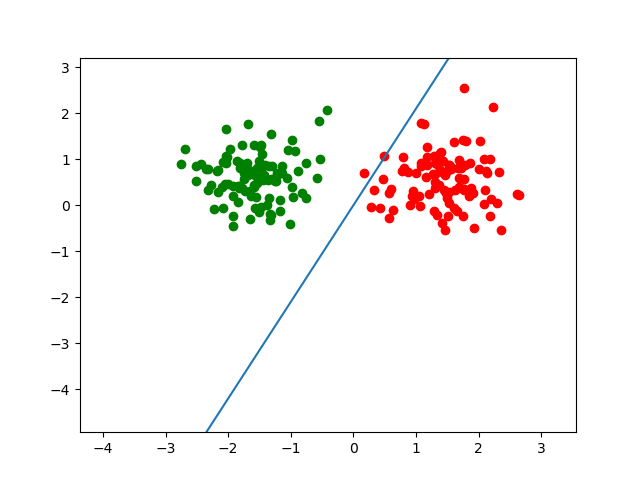
\includegraphics[width=\textwidth]{Labs/Lab 1/Lab 1a/Results/perceptron-linearly-seperable.png}
        \caption{Perceptron rule}
        \label{fig:Perceptron}
    \end{subfigure}
    \caption{Decision Boundary for Delta rule and Perceptron Rule}
    \label{fig:Decision Boundary}
\end{figure}\\
\textbf{Removing Bias check: }we also removed the bias to check how well delta rule converges. This can be seen in figure \ref{fig:DeltaRule-NoBias}
\begin{figure}[htb]
    \centering
    \begin{subfigure}{0.4\textwidth}
        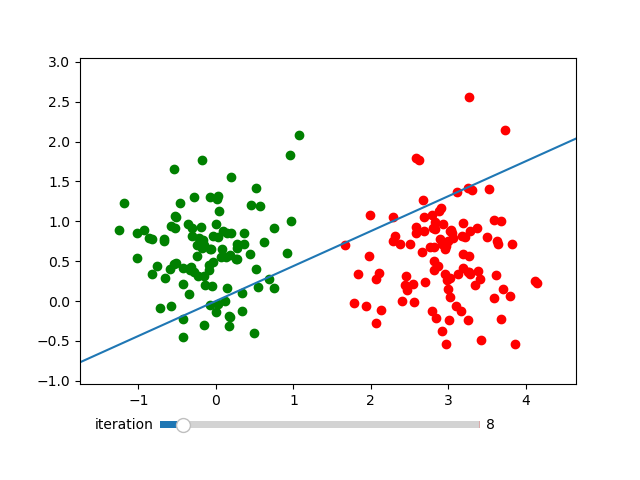
\includegraphics[width=\textwidth]{Labs/Lab 1/Lab 1a/Results/Delta-linear-seperable-NO-BIAS.png}
        \caption{Delta rule with 8 iterations}
        \label{fig:Delta Rule without bias, iteration 8}
    \end{subfigure}
    \hfill
    \begin{subfigure}{0.4\textwidth}
        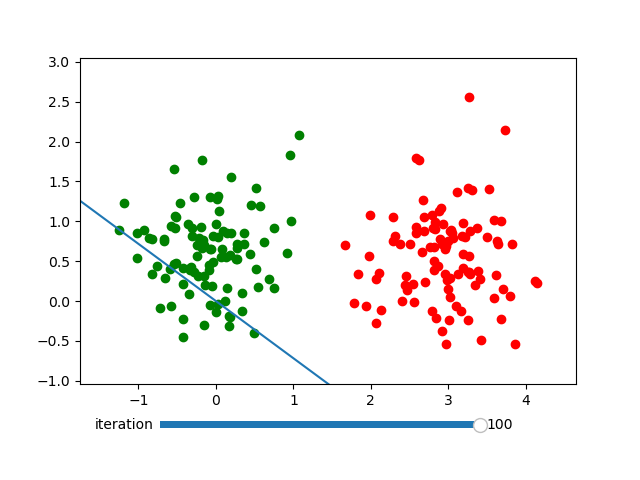
\includegraphics[width=\textwidth]{Labs/Lab 1/Lab 1a/Results/Delta-linear-seperable-NO-BIAS-ITERATION100.png}
        \caption{Delta rule with 100 iterations}
        \label{fig:Perceptron}
    \end{subfigure}
    \caption{Decision Boundary for Delta rule without bias }
    \label{fig:DeltaRule-NoBias}
\end{figure}
The decision boundary passes through origo regardless if it is not the optimal solution. The slope changes to become as optimal as possible. The bias simply changes the "starting" position of the slope which makes it easier to find the optimal decision boundary. 

\newpage
\textbf{Batch versus sequential learning:} Lastly we compared sequential versus batch learning. They converge to the same result however batch makes the changes faster after each iteration
\begin{figure}[htb]
    \centering
    \begin{subfigure}{0.4\textwidth}
        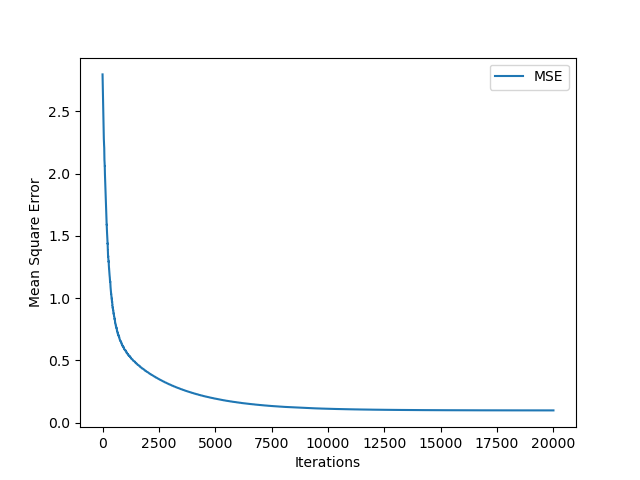
\includegraphics[width=\textwidth]{Labs/Lab 1/Lab 1a/Results/delta-linear-seperable-bias-sequential.png}
        \caption{Delta rule with sequential learning}
        \label{fig:Delta Rule with sequential learning}
    \end{subfigure}
    \hfill
    \begin{subfigure}{0.4\textwidth}
        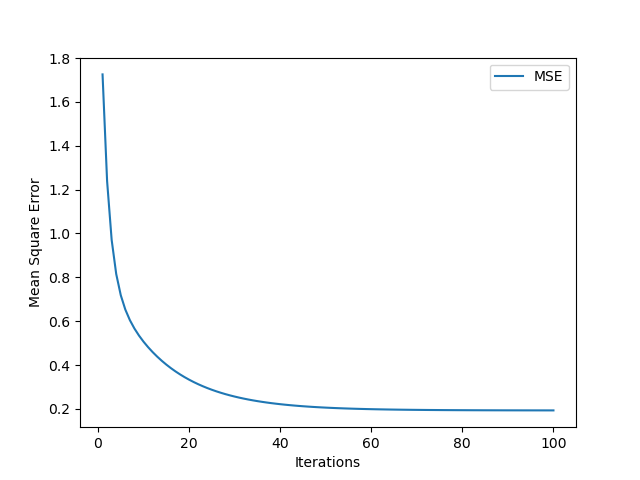
\includegraphics[width=\textwidth]{Labs/Lab 1/Lab 1a/Results/delta-linear-seperable-bias-BATCH.png}
        \caption{Delta rule with batch learning}
        \label{fig:DeltaRule with batch learning}
    \end{subfigure}
    \caption{Mean square error comparison of online and sequential learning}
    \label{fig:DeltaRule-NoBias}
\end{figure}


\subsection{Classification of data that are not linearly separable}
We created a dataset that is not linearly separable by using the same method as in the assignments above, moving the means of the two clusters closer together. That way the clusters overlap, and no longer are linearly separable. A picture of this new set of data points can be seen below.
\begin{figure}[htb]
    \centering
    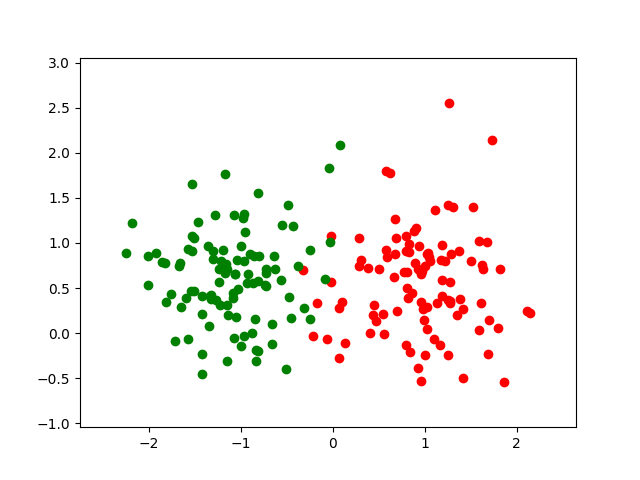
\includegraphics[width=0.8\textwidth]{Labs/Lab 1/Lab 1a/Results/overlapping_dataset.png}
    \caption{Data set that is not linearly separable}
    \label{fig:enter-label}
\end{figure}
First we tried fitting the single layer Perceptron using the Percepton learning algorithm. We expected that this would not work since it is only guaranteed that it converges if the dataset is linearly separable. Our simulations confirmed this. We tried fitting this Perceptron using the Perceptron learning rule. We calculated the mean square error in the same way as is done when using the Delta learning to get a glimpse into the error of the model. The model does not converge.

\begin{figure}[htb]
    \centering
    \begin{subfigure}{0.4\textwidth}
         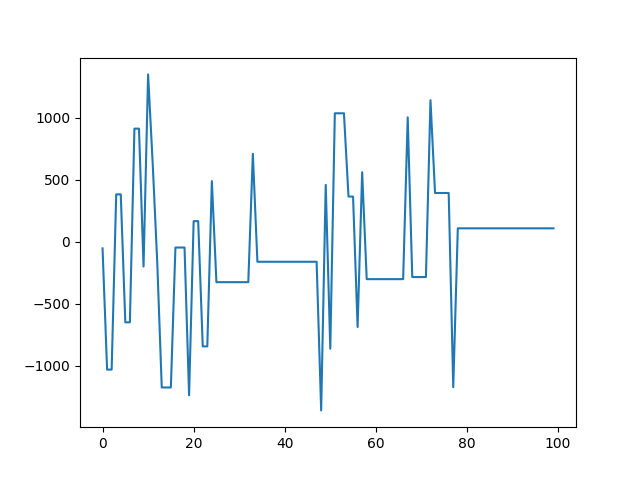
\includegraphics[width=\textwidth]{Labs/Lab 1/Lab 1a/Results/perceptron-training-error-convergence.png}
        \caption{Training error when using Perceptron}
        \label{fig:Perceptron-training-error}
    \end{subfigure}
    \hfill
    \begin{subfigure}{0.4\textwidth}
        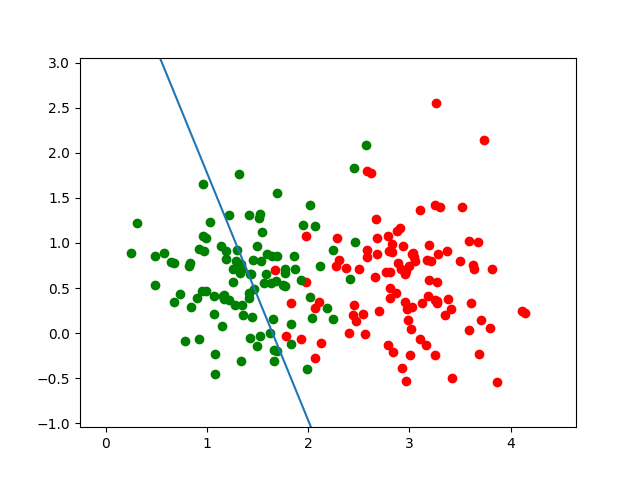
\includegraphics[width=\textwidth]{Labs/Lab 1/Lab 1a/Results/perceptron-decision-boundary-not-separable.png}
        \caption{Decision boundary obtained with perceptron learning}
        \label{fig:decision-boundary}
    \end{subfigure}
\end{figure}

The training error never reaches a point where it is stable. This makes sense since there will always be a point that is misclassified. When the training algorithm reaches that point it moves the boundary in a such a way that it will be on the correct side of the boundary. That will make another point misclassified and therefore this boundary will always keep on moving to make the current point correctly classified. An illustration of this can be seen below.

An illustration of how the decision boundary differs and is not stable can be seen in the two figures. They show how the decision line changes even after ten thousand iterations. In the first picture, we see a line, and after 10000 iterations, and in the second figure, we see another line that is different from the first one. It confirms the theory that the perceptron rule does not converge.   

We used a single layer Perceptron, trained using the Delta learning rule to classify this. We expected the learning algorithm to converge like it should, when using appropriate learning rate. As it turned out the algorithm did converge and we obtained the decision boundary shown in the picture below. The other picture shows how the training error developed through the training. It decreases fast in the beginning until it reaches convergence.

 
\begin{figure}[htb]
    \centering
    \begin{subfigure}{0.4\textwidth}
        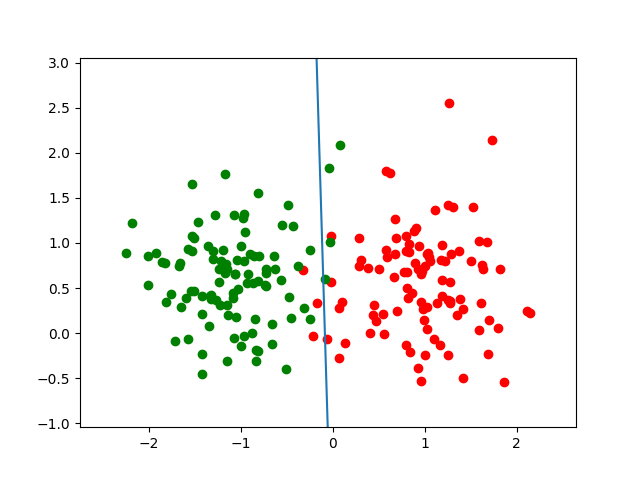
\includegraphics[width=\textwidth]{Labs/Lab 1/Lab 1a/Results/decicion-boundary-not-separable.png}
        \caption{Decision boundary on data set that is not linearly separable with Delta rule}
        \label{fig:Decision-boundary-not-linearly-separable}
    \end{subfigure}
    \hfill
    \begin{subfigure}{0.4\textwidth}
        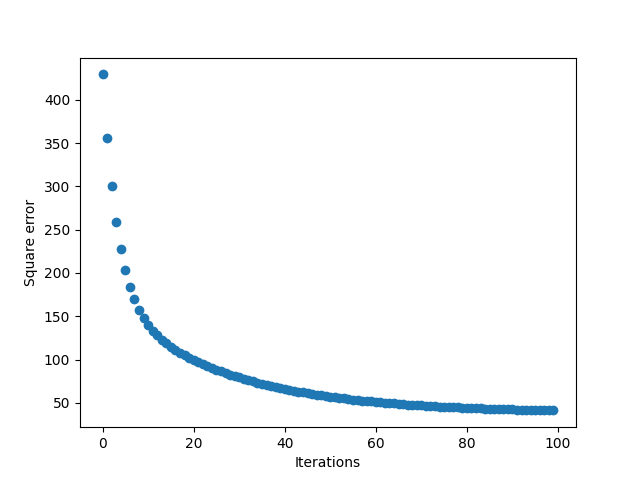
\includegraphics[width=\textwidth]{Labs/Lab 1/Lab 1a/Results/error-convergance.png}
        \caption{Delta rule with 100 iterations}
        \label{fig:Error-convergance}
    \end{subfigure}
\end{figure}



\begin{figure}[htb]
    \centering
    \begin{subfigure}{0.4\textwidth}
        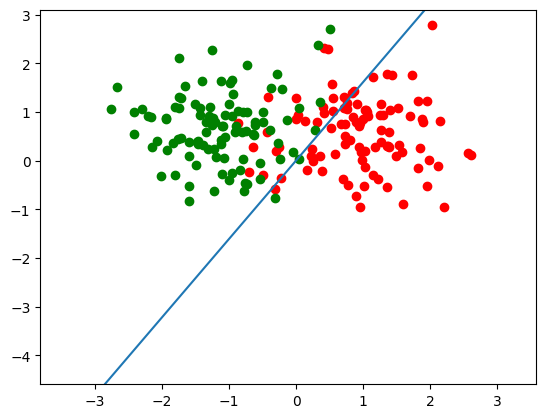
\includegraphics[width=\textwidth]{Labs/Lab 1/Lab 1a/Results/p_non_linear10000.png}
        \caption{Decision boundary on data set that is not linearly separable  using perceptron learning rule after 10000 iterations}
        \label{fig:Decision-boundary-not-linearly-separable}
    \end{subfigure}
    \hfill
\end{figure}

\begin{figure}[htb]
    \centering
    \begin{subfigure}{0.4\textwidth}
        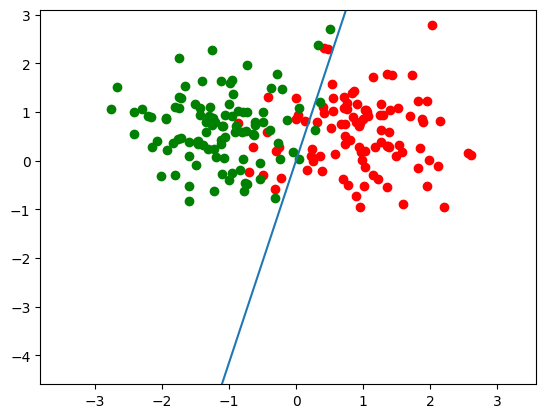
\includegraphics[width=\textwidth]{Labs/Lab 1/Lab 1a/Results/p_non_linear11000.png}
        \caption{Decision boundary on data set that is not linearly separable  using perceptron learning rule after 11000}
        \label{fig:Decision-boundary-not-linearly-separable}
    \end{subfigure}
    \hfill
\end{figure}







\section{Final remarks \normalsize{\textit{(ca. 0.5 page)}}} 
Overall, the lab was interesting as it helped us implement the theoretical concepts we learned from the lectures and see a practical example of how the classification task could be conducted using the perceptron implementation. It was also beneficial for our learning to use different approaches, the perceptron learning rule, and the delta rule, to classify the data and see which algorithm converges faster. One question could be asked if it is sufficient to use only one perceptron to classify binary data in real live implementation. Or the use of only perception is just for learning purposes and not used in practical examples. 
\end{document}
